\documentclass{article}
\usepackage{graphicx}
\usepackage{float}
\usepackage{amsmath}
\usepackage{lastpage}
\usepackage[stable]{footmisc}
\usepackage[margin=0.85in]{geometry}
\usepackage{fancyhdr}
\pagestyle{fancy}
\lhead{CSC373 Summer 2015}
\chead{Tutorial 9}
\rhead{TA: Eric Zhu}
\cfoot{Page \thepage~of~\pageref{LastPage}}
%\setlength{\parindent}{0pt}
\begin{document}

In this tutorial let's look at some examples of reductions for
NP-Completeness proof.

\section{VERTEX-COVER $\rightarrow$ CLIQUE \footnote{Based on 35.5 of {\it Introduction to Algorithms
2nd Edition} by Cormen, Leiserson, Rivest, and Stein}}

Recall that a {\bf vertex cover} is a subset of vertices that covers all the 
edges in a graph.
Formally, given an undirected graph $G = (V, E)$, a vertex cover is a subset
$V' \subseteq V$ such that if $(i, j)$ is an edge of $G$, then either
$i \in V'$ or $j \in V'$ (or both).
The decision problem, VERTEX-COVER, is to determine whether a graph has a
vertex cover of a given size $k$.
From the lecture, we know that VERTEX-COVER is NP-Complete, by
reducing 3SAT to VERTEX-COVER. 

A {\bf clique}, on the other hand, 
is a subset of vertices that are all directly connected.
Formally, given an undirected graph $G = (V, E)$, a clique is a subset 
$V' \subseteq V$ of vertices, each pair of which is connected by an edge in E.
The decision problem, CLIQUE, is to determine whether a clique of size $k$
exists in a graph.
Here, we want to prove that CLIQUE is also NP Complete, by reduction from
VERTEX-COVER.

Before we do the reduction, we need to first prove that CLIQUE $\in$ NP.
Recall that all problems in NP must be verifible in polynomial time.
Can we check the solution to CLIQUE in polynomial time?
Suppose we are given a graph $G = (V, E)$ and an integer $k$, and we 
have a solution $V' \in V$. We first check whether the size of $V'$ is
$k$, that is, $|V'| = k$. Then for every pair of vertices $u, v \in V'$,
check whether the edge $(u, v)$ is in $E$, 
or there exist an edge between $u$ an $v$.
The first check can be completed in $|V'|$ steps and the second check in
$|V'|^{2}$ steps. Thus the verification can be completed in $O(n^2)$ time,
and CLIQUE $\in$ NP.

Now we want to show that VERTEX-COVER can be reduced to CLIQUE.
Since we already know that VERTEX-COVER is NP Complete, if it can be reduced
to CLIQUE, then CLIQUE must also be NP Complete.

The reduction is brilliant: given an undirected graph $G = (V, E)$, we define
the {\bf complement} of $G$ as $\overline {G} = (V, \overline{E})$, where
$\overline{E} = \{(u,v) : u, v \in V, u \ne v, (u, v) \notin E\}$. Essentially,
$\overline{G}$ has the same set of vertices as $G$, none of the edges in
$G$, and all the edges that do not exist in $G$.
The beautiful part is: if there exist a clique $V'$ in $\overline{G}$, 
then $V - V'$ is a vertex cover in $G$.
The algorithm for VERTEX-COVER($G$, $k$) by reduction to CLIQUE goes as follows:
\begin{enumerate}
\item Given a graph $G = (V, E)$ and integer $k$
\item Generate the complement graph $\overline{G} = (V, \overline{E})$
\item Solve the problem CLIQUE($\overline{G}$, $|V|-k$)
\item If there is a solution, return Yes, else return No
\end{enumerate}

\begin{figure}[H]
\centering
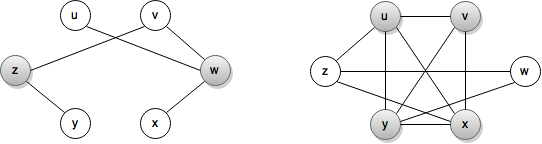
\includegraphics[width=0.5\textwidth]{clique_to_vertex_cover.png}
\caption{To the left, it is a graph $G = (V, E)$
	with vertex cover $V - V' = \{w, z\}$.
	To the right, it is the complement $\overline{G}$ with clique
	$V' = \{u, v, x, y\}$.}
\end{figure}

To prove this reduction is correct, we need to show two things:
\begin{itemize}
\item If there is a solution to VERTEX-COVER($G$, $k$), then there must
	be a solution to CLIQUE($\overline{G}$, $|V|-k$)
\item if there is a solution to CLIQUE($\overline{G}$, $|V|-k$), 
	then there must be a solution to VERTEX-COVER($G$, $k$)
\end{itemize}

First, suppose that $G$ has a vertex cover $V' \subseteq V$, where
$|V|' = k$. Then, for all $u, v \in V$, if $(u, v) \in E$,
then $u \in V'$ or $v \in V'$ or both, since the vertex cover must 
cover all edges. The contrapositive of this is that for all $u,v \in V$,
if $u \notin V'$ and $u \notin V'$, then $(u, v) \notin E$ and thus 
$(u,v) \in \overline{E}$. This is saying that for any pair of vertices
that are both not in the vertex cover $V'$ of $G$, 
there is an edge between them in $\overline{G}$. 
The union of all pairs of vertices that are all not in $V'$ is simply
$V - V'$. Thus, $V-V'$ is a clique in $\overline{G}$, by definition,
and $V-V'$ has size $|V| - k$.

Conversely, suppose that $\overline{G}$ has a clique $V' \subseteq V$, with
$|V'| = |V| - k$. Let $(u, v)$ be any edge in $E$. Then, $(u, v) \notin
\overline{E}$, which implies that at least one of $u$ or $v$ does not belong
to $V'$, since every pair of vertices in $V'$ is connected by an edge of
$\overline{E}$. Consequently, at least one of $u$ or $v$ is in $V-V'$.
This causes the edge $(u, v)$ to be covered by $V-V'$.
Since we chose $(u, v)$ arbitrarily from $E$, every edge in $E$ is covered
by $V-V'$. Therefore, the set $V-V'$ is a vertex cover of $G$, with size
$k$.

We have proven that VERTEX-COVER can be reduced to CLIQUE. However, can
the reduction be done in polynomial time? To generate the complement graph,
we only need a single scan over all pairs of vertices in the original graph,
and generate an edge if there is not edge between any pair.
This operation can be done in polynomial time.
Since VERTEX-COVER can be reduced to CLIQUE in polynomial time, 
CLIQUE $\in$ NP and VERTEX-COVER is NP-Complete, CLIQUE is also NP-Complete.

\section{VERTEX-COVER $\rightarrow$ SET-COVER}

A {\bf set cover} is a subset of subsets $S_1, S_2, \dots, S_n$ 
of a finite set $U$, such that their union is $U$.
A decision problem SET-COVER is to determine whether there exist a set cover
of size $k$ given $U$ and the subsets $S_1, S_2, \dots, S_n$.
There is a set cover with size $k=2$ in the example below, can you see it?
\begin{equation}
\begin{split}
	U &= \left\{1,2,3,4,5,6,7,8\right\} \\
	S_1 &= \left\{ 1,2,3,4 \right\} \\
	S_2 &= \left\{ 5,6,7,8 \right\} \\
	S_3 &= \left\{ 3,4,5,6 \right\}\\
	k &= 2
\end{split}
\end{equation}

To prove SET-COVER is NP Complete, we first need to show that SET-COVER $\in$
NP. A verification algorithm takes an instance SET-COVER($U$, $\left\{ S_1,
S_2, \dots, S_n\right\}$, $k$) and a solution $S$ as inputs.
First it check the size of $S$ is $k$. Then, it iterates through all elements 
of all subsets in $S$, and mark each element as seen. Once finished, check if 
all the elements in $U$ have been seen. Since both steps can be completed in
polynomial time with respect to the size of the inputs, the verification can
be done in polynomial time. Thus SET-COVER $\in$ NP.

Next, let's prove SET-COVER is NP-Complete by proving it can be reduced from
VERTEX-COVER. Suppose we are given a problem instance VERTEX-COVER($G$, $k$)
and $G = (V, E)$. We can construct an instance of SET-COVER as follows:
\begin{enumerate}
\item $U = E$ - let the set of all edges be $U$.
\item $S_i = \left\{ (u, v) \in E : u = i~or~v = i  \right\} \forall i \in V$
	- create a subset $S_i$ for every vetex i, and let it be all the edges 
	incident to $i$.
\item $k = k$ - set the problem to find vertex cover of size $k$.
\end{enumerate}
The vertices corresponding to the subsets in the subset cover of $U$ will be 
the vertex cover of $G$.

Let's prove the reduction is correct. Suppose there is a solution to
VERTEX-COVER($G$, $k$). Let it be $V'$ with size $k$. 
Then the vertices in $V'$ covers all
the edges in $E$. Since any subset $S_i$ is the set of edges incident on vertex
$i$, the union of all $S_i$ such that $i \in V'$ must contains all the edges
in $E$. Since all the edges in $E$ forms the set $U$, 
$\left\{ S_i : i \in V \right\}$ is a set cover of $U$, with size $k$.

Conversely, suppose there is a solution to the SET-COVER($U$, $\left\{ S_1,
S_2, \dots, S_n\right\}$, $k$). Let it be 
$S = \left\{ S_1, S_2, \dots S_k \right\}$ with out loss of generality.
Then $S_1 \cup S_2 \cup \dots \cup S_k = U$. Since $E = U$, $S$ covers all
edges in $E$. Since each $S_i \in S$ are the edges incident on vertex $i$, 
the vertices $\left\{ i : S_i \in S \right\}$ form a vertex cover of $G$,
with size $k$.

Lastly, the reduction can be done in polynomial time with respect to the inputs, 
because it only requires scanning all the edges once to create the subsets
$S_i$s and $U$. Therefore, SET-COVER is NP-Complete.

\end{document}

